\documentclass[a4paper,11pt,headings=small]{article}

\usepackage[T1]{fontenc}
\usepackage[pdftex]{graphicx}
\usepackage{dblfloatfix}
\usepackage{multicol}
\usepackage{cite}
\usepackage{pdfpages}
\usepackage{cite}
\usepackage{tikz}
\usepackage{multirow}
\usepackage[english]{babel}
\usepackage{float}
\usepackage{mathcomp}
\graphicspath{{images/}}
\usepackage{amsmath}
\usepackage{amsfonts}
\usepackage{amssymb}
\usepackage{fouridx}
\usepackage{cancel}	
\usepackage{setspace}
\usepackage[ansinew]{inputenc}
\usepackage[format=plain,font=small,margin=10pt,labelfont=bf,labelsep=quad]{caption}
\usepackage{subcaption}
\usepackage{ipa}
\usepackage{a4wide}
\usepackage{titlesec}
\usepackage{array}
\usepackage{booktabs}
\usepackage[top=3.0cm, bottom=3.0cm, left=2cm, right=2cm]{geometry}
\sloppy
\usepackage{fancyhdr}
\usepackage{verbatim}

\usepackage{hyperref}
\hypersetup{colorlinks=true}

\setlength{\columnsep}{1cm}
\DeclareMathOperator*{\argmax}{arg\,max}

\begin{comment}
NOTES/TODO

Lessons Learned:
* Covariance matrix is CRUCIAL. In fact, it's everything.
  * Should capture frames of the progression from bad to good kernel fn.
* Author was doing everything in pixels! This screws up my hyperparameters!
* How far into future to predict.
* How to get MAP (take the mean).
* Correspondence is key. In both cases, fixed major issues.

To Include:
* Homography transform
* Kernel & hyperparameter definition
	* Charts describing kernel
* Final MAP calculation (mean weighted by IP)
* Performance metric (path length + safety calculation)
* Final results (over how many frames? for different particle swarm sizes?)

\end{comment}

\begin{document}

%\twocolumn[
%  \begin{@twocolumnfalse}
  \vspace{-1cm}
	\begin{flushright}
	February 6, 2014\\
	\end{flushright}
	\vspace{0.6cm}
	\LARGE{\textbf{Robot Navigation in Dense Human Crowds}\\[0.2cm] Final Report}\\\\ \\
	\large{Neil Traft\\[0.1cm] University of British Columbia}		 	 	\vspace{0.6cm}
%\end{@twocolumnfalse}
%]


\pagestyle{fancy}
\fancyhf{}
\fancyhead[L]{Robot Navigation in Dense Human Crowds}
\fancyhead[R]{Neil Traft --- \thepage}

\pagenumbering{arabic}
\setcounter{page}{1}

%\onehalfspacing
\renewcommand{\thesection}{\Roman{section}}
\thispagestyle{empty}

\newcommand{\f}{\mathbf{f}}
\newcommand{\fr}{\f^{(R)}}
\newcommand{\fati}{\f^{(i)}}
\newcommand{\fatj}{\f^{(j)}}
\newcommand{\samplej}{(\fatj)_i}
\newcommand{\z}{\mathbf{z}}
\newcommand{\ztot}{\z_{1:t}}
\newcommand{\pos}{\mathrm{pos}}
\newcommand{\post}{\pos^{(i)}_t}

\section*{Overview}
\quad In their 2010 IROS publication \cite{Trautman2010}, Trautman and Krause develop a path planning algorithm that is safe and yet does not suffer from the ``freezing robot problem'' (FRP). Their method consists of a model of crowd interaction combined with a particle-based inference method to predict where the crowd (and the robot) should be at some time $t+1$ in the future. The idea is that if one can develop a reliable model of intelligent agents in a crowd, and include the robot as just another of those intelligent agents, then the predictions of the model yield the robot's future path.

\subsubsection*{Interacting Gaussian Processes}
\quad The crowd interaction model is a nonparametric stochastic model based on Gaussian processes, dubbed \emph{Interacting Gaussian Processes} (IGP). In IGP, the actions of all agents, including the robot, are modeled as a joint distribution:
$$p(\fr,\f|\ztot)$$
where $\fr$ is the robot's trajectory over $T$ timesteps, $\f$ is the set of all human trajectories, and $\ztot$ is the set of all observations up to the current time point. For the purposes of this algorithm, observations of human and robot position are taken to be more or less perfect, since we are only trying to solve the navigation problem, not situational awareness.

At each timestep, each agent's new position is represented as a random variable from a probability distribution. It is important to note that this distribution is \emph{not} Gaussian, due to two major additions to avoid the uncertainty explosion which leads to the FRP (see Figure \ref{uncertainty}).

First, goal information is given as a final ``observation'' at time $T$, resulting in the full set of observations $\z_{1:t,T}$. The robot's goal, $y_T^{(R)}$, is known and can be added with good confidence. The goals of other agents can be omitted or can be added with a large confidence interval, to encode how uncertain we are about the goal.

The second addition IGP makes to standard Gaussian processes is the inclusion of an ``interaction potential:''
$$ \psi(\fr,\f) = \prod_{i=1}^n \prod_{j=i+1}^n \prod_{\tau=t}^T \left( 1 - \alpha \exp\big(-\frac{1}{2h^2}|\fati_{\tau} - \fatj_{\tau}|\big) \right)$$

In essence, this potential grows very small whenever two agents $i$ and $j$ become very close at any time $\tau$. This has the result that any set of paths where agents become too close is treated as very unlikely. The parameter $h$ controls the desired ``safety distance'' and $\alpha \in [0, 1]$ controls the ``repelling force''. Thus, the final posterior is given as:
$$ p_{IGP}(\fr,\f | \ztot) = \frac{1}{Z} \; \psi(\fr,\f) \prod_{i=1}^n p(\fati | \ztot) $$

% What is Z?

The above is a nonlinear, multimodal distribution, so it can't be sampled directly. Instead, we sample from Gaussian priors $p(\fati|\ztot)$ and resample weighted by our desired distribution (a particle filter). This is described in the next section.

\begin{figure}[h]
\centering
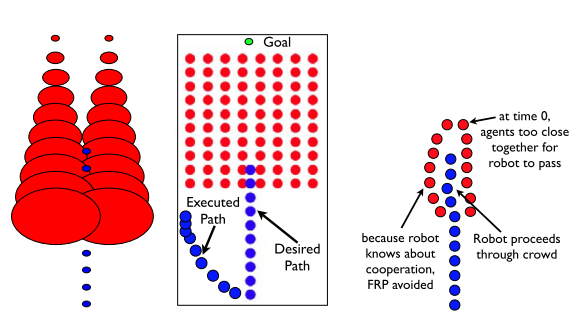
\includegraphics[width=.75\textwidth]{uncertainty-explosion.png}
\caption{Diagrams taken from \cite{Trautman2010} describing the uncertainty explosion which leads to the Freezing Robot Problem. \textbf{Left:} Depicts the uncertainty explosion in standard motion models, where each agent's trajectory is \emph{independent} from the others. \textbf{Middle:} A demonstration of why even \emph{perfect} prediction, devoid of uncertainty, can still lead to the FRP. In crowded environments, \emph{all} paths can have a high cost function, leading to extreme evasive maneuvers or freezing. \textbf{Right:} The ideal model, based on the insight that intelligent agents engage in \emph{cooperative} collision avoidance.}
\label{uncertainty}
\end{figure}

\subsubsection*{Importance Sampling}
\quad Now that we have a model, we wish to sample from it and take the mean as the desired path. Since we can't sample from it directly, we instead use the \emph{importance sampling} technique which is widely used in particle filters. Each sample is weighted by the ratio of the IGP to the basic GP (i.e. the Gaussian distribution, without the interaction potential):
$$ w_i = \frac{p_{IGP}}{p_{GP}} = \frac{p_{IGP}((\fr,\f) | \ztot)}{\prod_{j=R}^n p(\samplej | \ztot)} = \frac{\psi((\fr,\f)_i) \prod_{j=R}^n p(\samplej | \ztot)}{\prod_{j=R}^n p(\samplej | \ztot)} = \psi((\fatj)_i)$$
where $\samplej$ is a single sample from the trajectory of agent $j$.

Given this formulation for $p_{IGP}$ and an appropriate weighting $w_i$ for each sample, we can now find the ideal paths:
$$ (\fr,\f)^* = \argmax\left( \sum_{i=1}^N w_i(\fr,\f)_i \right) $$
where $(\fr,\f)_i$ is a set of samples from the Gaussian processes $(\fatj)_i \sim \textrm{GP}(\fatj, m_t^{(j)}, k_t^{(j)})$ (detailed equations for the mean and covariance matrix can be found in the original paper). The total number of samples is $N$ and we take the robot's next position to be $\fr_{t+1}$.

\section*{Current Status}
\quad Currently I have downloaded the dataset that will be used for my simulations and begun visualization of the data (see Figure \ref{bug}). I found the only reasonable way to create visualizations on top of video frames in Python was actually to use the OpenCV library\cite{opencv}, so this has been downloaded and installed. Currently it's only being used for video processing and visualization, not for any of the vision algorithms it provides.

\subsection*{The Dataset}
\quad The dataset to be used is the ETH Walking Pedestrians (EWAP) dataset from \cite{Pellegrini2009}. It has been downloaded from \cite{dataset}.

The dataset contains two annotated videos of pedestrian interaction captured from a bird's eye view. Only one of these was used in Trautman's paper, a sequence acquired from the top of the ETH main building, Zurich, in 2009. The film captures people entering to and exiting from the main entrance of the building, such that agents in the image have two main goals: either their goal is a point at the bottom of the image (the entrance), or they are emerging from the entrance and their goal is somewhere along the top of the image (the street).

The main annotations are a matrix where each row has the format:
\begin{verbatim}
        [frame_number pedestrian_ID pos_x pos_z pos_y v_x v_z v_y]
\end{verbatim}

Thus for each frame $t$ we have potentially multiple pedestrian observations $\post$, and this forms our observation at time $t$:
$$ \z_t = \pos^{(1:n)}_t $$
where one of the $n$ pedestrians is chosen to represent the robot $R$.

The \texttt{pos\_z} and \texttt{v\_z} (direction perpendicular to the ground) are not used in the annotations. The velocities will not be used by the IGP algorithm altogether; its only observations are positions at each timestep.

The positions and velocities are in meters and were obtained with a homography matrix $H$, which is also provided with the annotations. To transform the positions back to image coordinates, it is necessary to apply the inverse homography transform:
$$ \fourIdx{m}{}{}{}\post = H_{mw}^{-1} \cdot \fourIdx{w}{}{}{}\post \qquad m = \mathrm{image}, w = \mathrm{world} $$

In addition to the main annotations, there is also a list of possible destinations. These must be transformed into image coordinates in the same way. These can be used as the set of possible goals that IGP uses to help reduce the uncertainty explosion. In actual implementation, the goals $y^{(i)}_T$ for each pedestrian $i$ are just observations at the final timepoint, $\z_T$.

This is just a set of possible goals; the method for choosing which pedestrian has which goal is flexible. The original paper does not detail how these goals are chosen, but \cite{Pellegrini2009} assigns each pedestrian the closest goal at each timepoint in their crowd interaction model. This is surprising to me, as it seems like this would pull the predictions in the exact opposite direction until the pedestrian gets to the middle of the image, but I'll start with it and refine it later if needed.

\subsection*{Next Steps}
\quad At present there is a problem with how I'm transforming pedestrian points into image space using the homography matrix. This affects only the visualization, as the path planner will work in world coordinates, but I will need to fix it before I can really tell what my algorithm is doing. It seems to be nearly correct, but needs to be normalized into some bounding box that isn't specified in the documentation for the EWAP dataset. An example of the bug is given in Figure \ref{bug}.

\begin{figure}[h]
\centering
\begin{subfigure}[b]{0.8\textwidth}
\centering
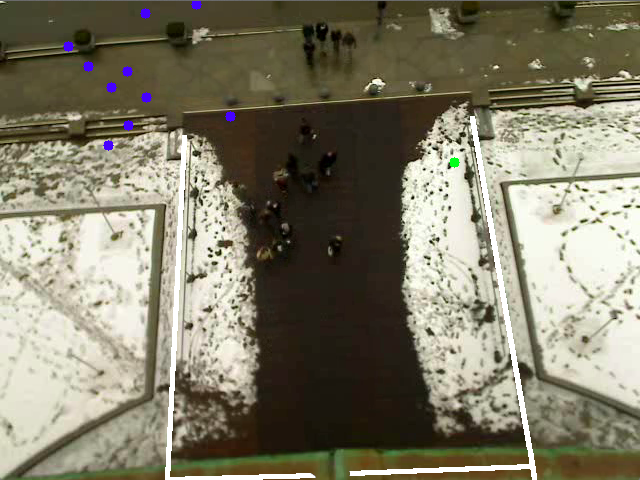
\includegraphics[width=\textwidth]{dataset-bug.png}
\caption{A sample frame from my current visualization.}
\label{a}
\end{subfigure}
\begin{subfigure}[b]{0.8\textwidth}
\centering
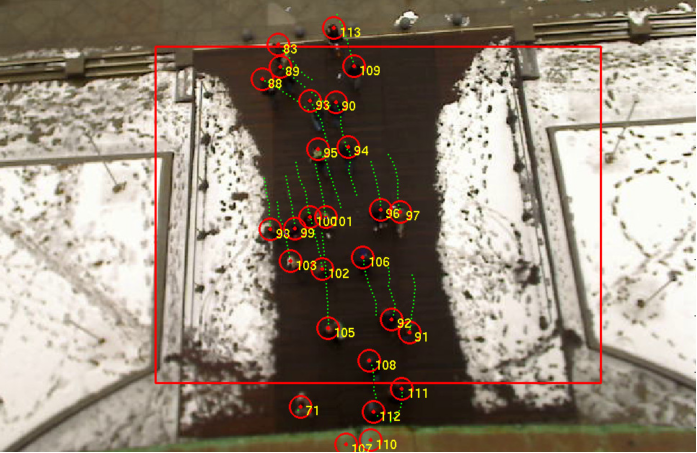
\includegraphics[width=\textwidth]{dataset-example.png}
\caption{A sample frame from the ETH paper.\cite{Pellegrini2009}}
\label{b}
\end{subfigure}
\caption{A sample frame from my (buggy) implementation (\ref{a}) compared with a correct implementation (\ref{b}). In the top image, blue dots mark pedestrians, white lines mark static obstacles, and green dots mark possible destinations. If examined closely, one can see the pedestrian markings in my video are correct in relation to each other, but appear scaled and translated within the image plane. The destinations appear to have the same issue (only one destination is visible but there are about 4 total).}
\label{bug}
\end{figure}

Once this is fixed, the visualization will be mostly complete, except that we will want to display positions from multiple timepoints, past and present.

After this I'll need to implement the algorithm as previously planned. I will choose particular time points at which to run IGP, and choose a particular pedestrian to represent the ``robot''. By evaluating IGP at this single time slice, and comparing it to the actual path taken by the pedestrian, we can evaluate the performance of the planner. We evaluate its performance based on $l$, the length of the path, and $s$, the minimum distance which the path ever comes within another pedestrian's path.

Once the algorithm is working correctly, there will be some final work tuning parameters and goals. I will have to tweak the parameters $\alpha$ and $h$ in the interaction potential, since the ones used for the original experiments are not directly given (though some suggestions are implied). I will also have to tweak the number of particles used for inference, though the paper does specify a range of $[100,5000]$ which should help. Finally, as discussed above, I may need to experiment with different methods of assigning goals to human agents in the scene.

% Include Timeline?

\bibliography{references}
\bibliographystyle{ieeetr}

\end{document}
